\paragraph{One-component interventions on copied witnesses.}
We reconstruct each original full inference cohort from its case/tape seeds
and recovered checkpoint SHA. The unchanged execution matches its stored
terminal colors, steps and status, and all actions match through the selected
intervention frame. At that frame only one candidate is replaced by a free
alternative; all other messages and first-stage tensors stay fixed and the
learned second exchange/COMMIT is recomputed. A separate control substitutes
exact confirmation on the unchanged proposals once. Neither intervention
changes a training run or any reported autonomous test.

\begin{figure}[htbp]\centering
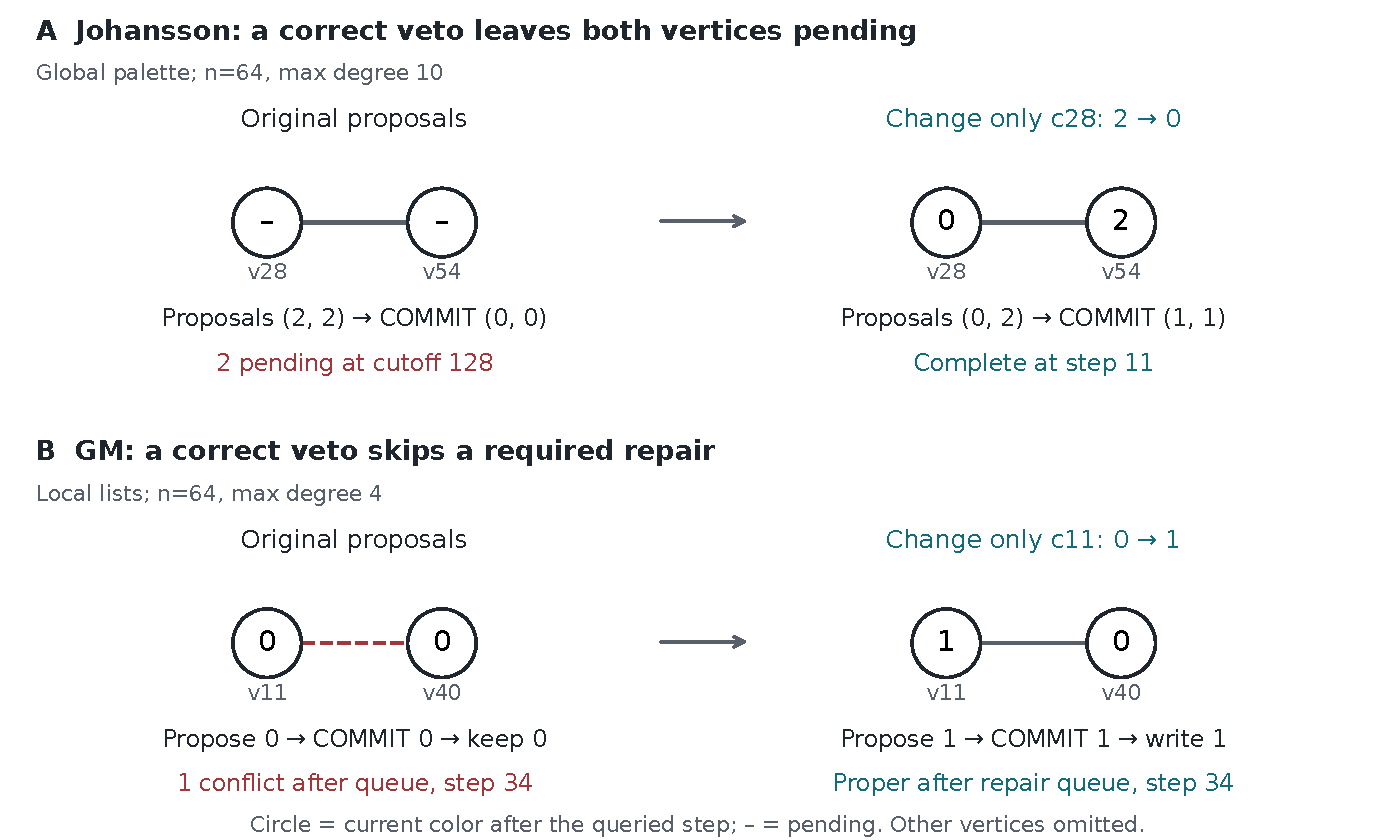
\includegraphics[width=\linewidth]{figures/revision-failure-mechanisms.pdf}
\caption{Two selected copied witness executions, showing local fragments
after one queried application. A: Johansson steps 10 to 11, with free colors
$\{0,2\}$ at both vertices. B: GM steps 32 to 33, with list $\{0,1\}$ at
the scheduled vertex 11; the dashed edge is an existing conflict. Changing
one proposal and recomputing learned COMMIT completes each copied run.
Exact-COMMIT substitution on unchanged proposals preserves both failures.
All other messages and first-stage tensors stay fixed at the intervention;
these cases do not estimate a population rescue rate. Full outcomes are
in Table~\ref{tab:rescues}.}
\label{fig:failure-mechanisms}
\end{figure}


These controls separate a proposal defect from an incorrect veto in the
selected states. Exact-COMMIT substitution is an identity at these already
correct vetoes, not an all-state oracle replacement or an audit of COMMIT
everywhere. The controls do not establish that changing the proposal module
would fix every failed execution, or that the first latent calibration
discrepancy caused the observed terminal failure.
